\begin{figure}[H]
  \centering
  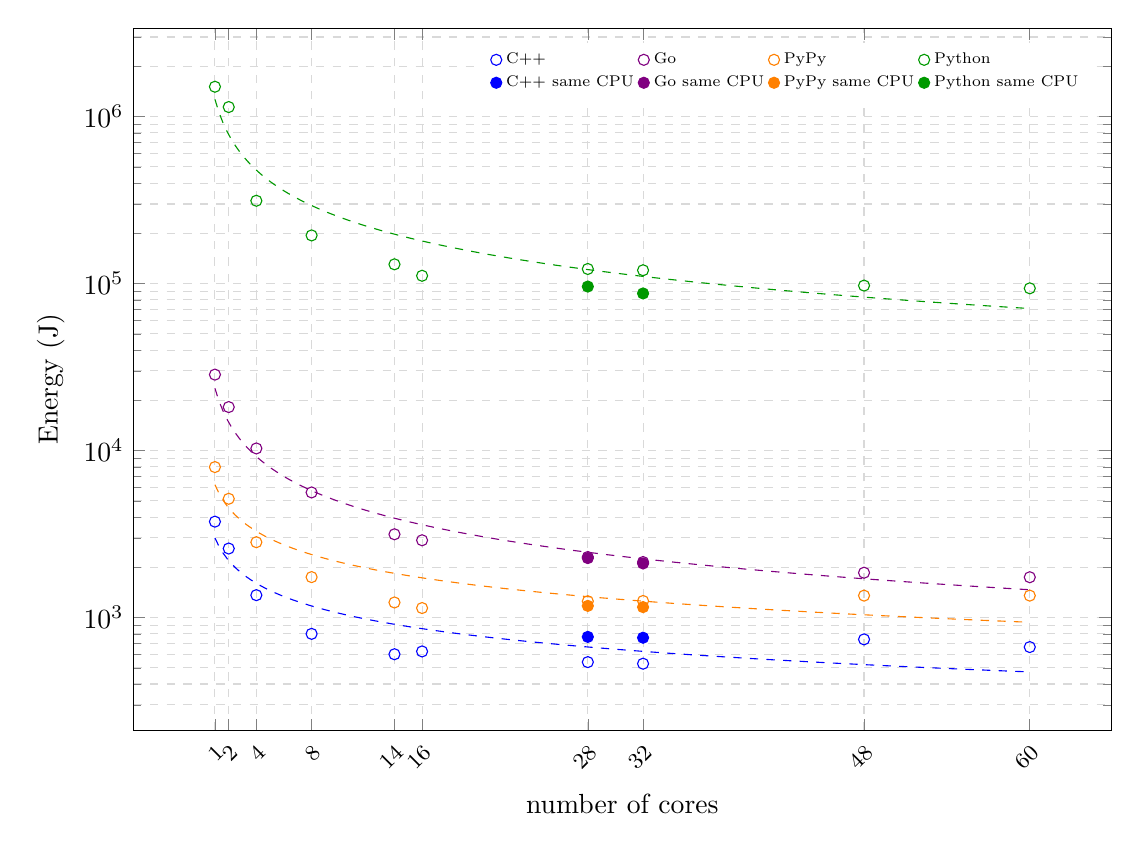
\begin{tikzpicture}
  \begin{semilogyaxis}[
      width=14cm,
      height=10.5cm,
      xlabel={number of cores},
      ylabel={Energy (J)},
      ymode=log,
      xmode=linear,
      grid=both,
      minor tick num=1,
      grid style={gray!30,dashed},
      xtick={1,2,4,8,14,16,28,32,48,60},
      x tick label style={
        font=\footnotesize,
        rotate=45,
        anchor=north east
      },
      legend style={
        at={(0.98,0.98)},
        anchor=north east,
        font=\scriptsize,
        nodes={scale=0.8,transform shape},
        draw=none
      },
      legend columns=2,
      transpose legend,
      legend cell align=left,
    ]

    %% C++ %%
    % open circles
    \addplot[
      blue,
      only marks,
      mark=o,
      mark options={draw=blue,fill=white}
    ] table[row sep=\\] {
      x    y \\
      1    3756.26  \\
      2    2591.91  \\
      4    1362.61  \\
      8    799.23   \\
      14   603.37   \\
      16   627.16   \\
      28   541.37   \\  
      32   529.61   \\  
      48   740.57   \\
      60   666.04   \\
    };
    \addlegendentry{C++}
    % filled circles at 28 & 32
    \addplot[
      blue,
      only marks,
      mark=*,
      mark options={draw=blue,fill=blue}
    ] table[row sep=\\] {
      x    y \\
      28   766.51   \\  
      32   757.79   \\  
    };
    \addlegendentry{C++ same CPU}
    % trendline, but do NOT add to legend:
    \addplot[
      blue,
      dashed,
      forget plot,
      domain=1:60,
      samples=200
    ] {3000 * x^(-0.4513)};

    %% Go %%
    \addplot[
      violet,
      only marks,
      mark=o,
      mark options={draw=violet,fill=white}
    ] table[row sep=\\] {
      x    y \\
      1    28522.69 \\
      2    18231.97 \\
      4    10304.27	\\
      8    5617.27  \\
      14   3155.30  \\
      16   2904.52  \\
      28   2306.35  \\
      32   2151.74  \\
      48   1856.93  \\
      60   1744.76  \\
    };
    \addlegendentry{Go}
    \addplot[
      violet,
      only marks,
      mark=*,
      mark options={draw=violet,fill=violet}
    ] table[row sep=\\] {
      x    y \\
      28   2271.71  \\
      32   2109.37  \\
    };
    \addlegendentry{Go same CPU}
    \addplot[
      violet,
      dashed,
      forget plot,
      domain=1:60,
      samples=200
    ] {23600 * x^(-0.6783)};

    %% PyPy %%
    \addplot[
      orange,
      only marks,
      mark=o,
      mark options={draw=orange,fill=white}
    ] table[row sep=\\] {
      x    y \\
      1    7972.65  \\
      2    5147.60  \\
      4    2828.21  \\
      8    1747.96  \\
      14   1232.03  \\
      16   1140.80  \\
      28   1252.93  \\
      32   1257.81  \\
      48   1354.03  \\
      60   1354.03  \\
    };
    \addlegendentry{PyPy}
    \addplot[
      orange,
      only marks,
      mark=*,
      mark options={draw=orange,fill=orange}
    ] table[row sep=\\] {
      x    y \\
      28   1175.52  \\
      32   1155.74  \\
    };
    \addlegendentry{PyPy same CPU}
    \addplot[
      orange,
      dashed,
      forget plot,
      domain=1:60,
      samples=200
    ] {6250 * x^(-0.4633)};

    %% Python %%
    \addplot[
      green!60!black,
      only marks,
      mark=o,
      mark options={draw=green!60!black,fill=white}
    ] table[row sep=\\] {
      x    y \\
      1    1510534.76 \\
      2    1141490.15 \\
      4    313537.85  \\
      8    194458.98  \\
      14   130506.94  \\
      16   111438.01  \\
      28   122384.40  \\
      32   120259.78  \\
      48   97331.00   \\
      60   93718.97   \\
    };
    \addlegendentry{Python}
    \addplot[
      green!60!black,
      only marks,
      mark=*,
      mark options={draw=green!60!black,fill=green!60!black}
    ] table[row sep=\\] {
      x    y \\
      28   96049.86 \\  
      32   87343.61 \\
    };
    \addlegendentry{Python same CPU}
    \addplot[
      green!60!black,
      dashed,
      forget plot,
      domain=1:60,
      samples=200
    ] {1.27e6 * x^(-0.7046)};

  \end{semilogyaxis}
\end{tikzpicture}
\caption{Energy consumption of the pkg (package, chips) server in Joules for different core configurations}
\label{fig:server-energy-pkg}
\end{figure}


\begin{table}
    \centering
    \begin{tabular}{lrrrr}
        \hline
        energy-pkg     & C++                & Go         & PyPy       & Python        \\
        \hline
        1              & 3,756.26            & 28,522.69   & 7,972.65   & \textbf{1,510,534.76}  \\
        2              & 2,591.91            & 18,231.97   & 5,147.60   & 1,141,490.15           \\
        4              & 1,362.61            & 10,304.27   & 2,828.21   &   313,537.85           \\
        8	             &   799.23 	         & 5,617.27    & 1,747.96   &	 194,458.98            \\ 
        14             &   603.37            & 3,155.30    & 1,232.03   &   130,506.94           \\
        16             &   627.16            & 2,904.52    & 1,140.80   &   111,438.01           \\
        28             &   \textbf{541.37}   & 2,306.35    & 1,252.93   &   122,384.40           \\
        28 same CPU    &   \textbf{766.51}   & 2,271.71    & 1,175.52   &   \textbf{96,049.86}   \\
        32             &   \textbf{529.61}   & 2,151.74    & 1,257.81   &   120,259.78           \\
        32 same CPU    &   \textbf{757.79}   & 2,109.37    & 1,155.74   &   \textbf{87,343.61}   \\
        48             &   740.57            & 1,856.93    & 1,354.03   &    97,331.00           \\
        60             &   666.04            & 1,744.76    & 1,354.03   &    93,718.97           \\
        \hline
    \end{tabular}
    \caption{Energy usage (pkg) by implementation and core count}
\label{tab:server-energy-pkg}
\end{table}
